\begin{surferPage}[Sextique à 30 pointes]{La Sextique de Barth à 30 Pointes}
    \`A la suite de la construction par Wolf Barth de la sextique ayant le plus grand nombre possible
    de singularités, $65$ (voir une autre surface de cette galerie) et
    de la construction par deux de ses étudiants en thèse d'autres surfaces ``record''
    de plus grand degrés, il s'intéressa au problème du nombre maximal
    de pointes sur des surfaces d'un degré donné.

   La construction de Barth de la sextique à $65$ singularités de type
    $A_1^{+-}$ (cônes doubles) peut être adaptée aux pointes, en en fournissant $30$ : 
    \[P_6 - \alpha \cdot K^3=0,\]
  où $P_6$ renvoie aux mêmes plans de symétrie de l'icosaèdre que pour
    l'autre Sextique de Barth, et où $K$ est
    à nouveau l'équation de la sphère unité :
    \vspace*{-0.4em}
    \begin{center}
      \begin{tabular}{c@{\ }c@{\ }c@{\ }c}
        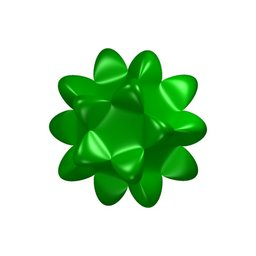
\includegraphics[height=1.2cm]{./../../common/images/barthsextic_30A2}
        &
        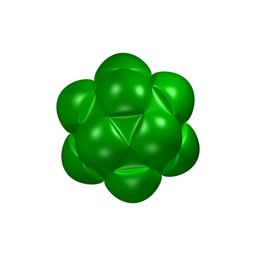
\includegraphics[height=1.2cm]{./../../common/images/barthsextic_30A2_3}
        &
        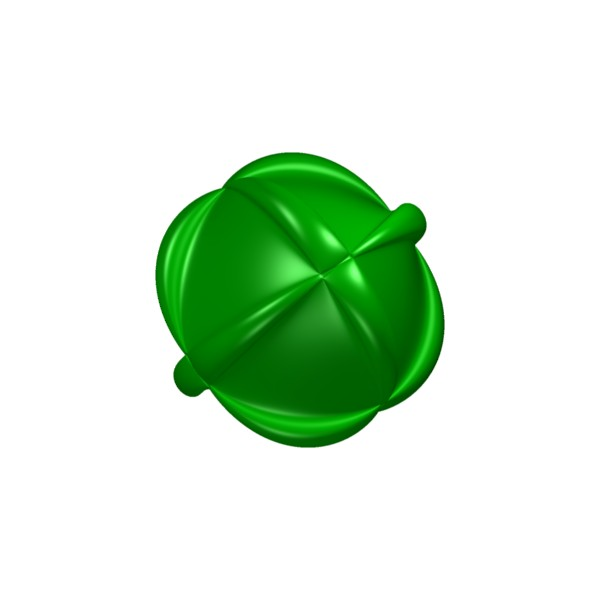
\includegraphics[height=1.2cm]{./../../common/images/barthsextic_30A2_5}
        &
        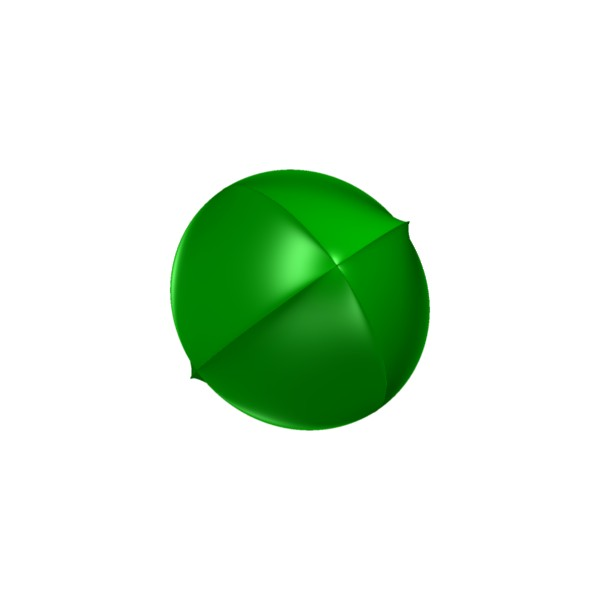
\includegraphics[height=1.2cm]{./../../common/images/barthsextic_30A2_6}
      \end{tabular}
    \end{center}    
    \vspace*{-0.3em}
     Il s'agit du record actuel du nombre de pointes réelles pour les
    sextiques, pour les pointes complexes, le record est de $36$.
\end{surferPage}
